\documentclass[11pt,a4paper]{article}
\usepackage[utf8]{inputenc}
\usepackage[T1]{fontenc}
\usepackage[english]{babel}
\usepackage{hyperref}
\usepackage{amsmath}
\usepackage{amsfonts, amsthm, bm}
\usepackage{mathrsfs}
\usepackage{graphicx}
\usepackage{amsthm}
\usepackage{newlfont}
\usepackage{color}
\usepackage{natbib}
\usepackage{float}
\usepackage{textcomp}


\textwidth=450pt\oddsidemargin=0pt

\renewcommand{\baselinestretch}{1,2}
\title{\Huge{\textbf{Study on Overfitting}} \\ 
                \vspace{5mm}
                \large{A review on Overfitting in Deep Learning  models}}
\author{Mattia Ceccarelli}
\date{June 2020}

\begin{document}
\maketitle

The project aim is to study how overfitting can represent a problem in common data analisys tasks and how to detect and avoid it in Deep Learning Applications.

The datasets used over the whole study are \textit{MNIST-784}, composed of $70.000$, $28 x 28$ grey-scale images containing hand-written digits; and \textit{CIFAR-10}, composed of $60.000$, $32 x 32$ colored images comprehensive of $10$ classes of objects.

The study will also focus on recent discoveries regarding overfitting in deep learning.

All the data obtained in the case of Deep Learning models are obtained by using the famous python library Tensorflow \cite{tf} 

\section*{Overfitting in data analysis}

In the context of data analysis overfitting is a common problem that arises from different factor. 
The main cause of overfitting is noise: indeed, by definition, an analytical or statistical model is "overfitted" when the outcome of the algorithm is overly affected by the noise in the data, which means the model begin to describe the random error in the data rather than the relationship between variables.

This ordinary but important flaw of machine learning and deep learning model brings a series of consequences that have as a secondary effect to reduce the effectiveness of the model, in particular in data it has never seen before: this phenomenon is called lack of Generalizations capabilities.

An example of overfitting in analytical method is shown in figure \ref{polyfit} found when using a simple polynomial fit on randomly generated data from $f(x) = 5 * sin(x * 9 / 10) + \nu$ where $\nu$ is a normally distributed random variable with $\mu = 0$ and $\sigma = 1$. The results obtained in the case of high order polynomial can be considered as a form of overfitting since the model tries to exactly fit every random  point.    

\begin{figure}[H]

 \centering
 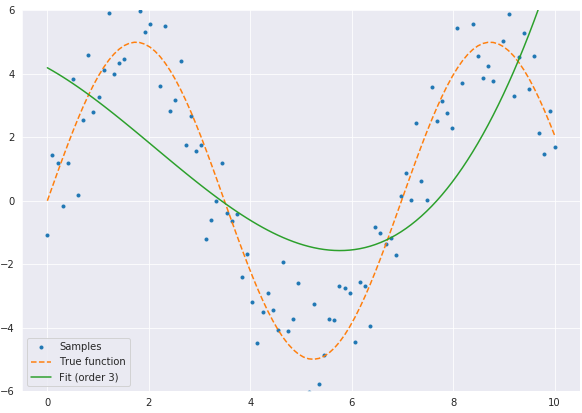
\includegraphics[scale=0.35]{../images/fit_nlinear_order3.png}
 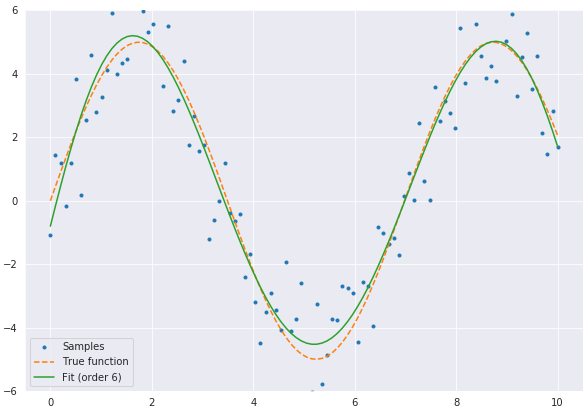
\includegraphics[scale=0.35]{../images/fit_nlinear_order6.png} \\
 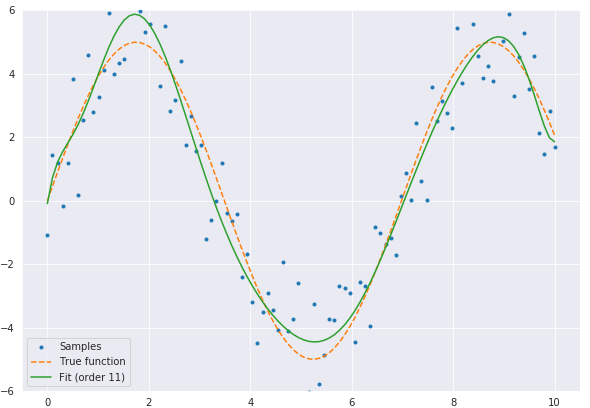
\includegraphics[scale=0.35]{../images/fit_nlinear_order11.png}
 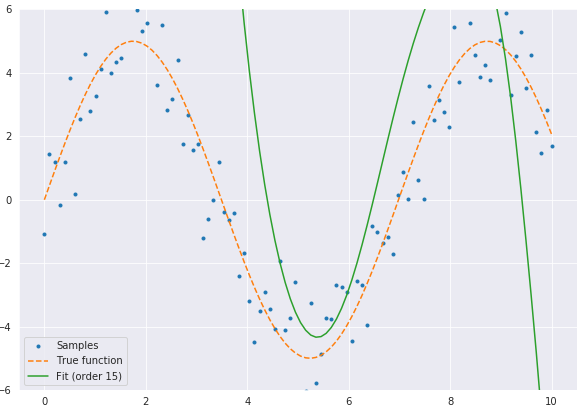
\includegraphics[scale=0.35]{../images/fit_nlinear_order15.png}
 \caption{\textit{The image shows in order from left to right and from up to down: underfitting of polynomial with order 3, best fit with polynomial of order 6, and overfitting with polynomial of order 11 and 15}}  
 \label{polyfit}
 
\end{figure}

Given the fact that noise can't be removed from data a priori, many different techniques has been developed to avoid overfitting. 
The most widely used is the simple divsion between training data and test data, which allow more control over the performances of the models. 
Figure \ref{scheme} shows some variation of the same concept: keep train and test data separated.
This greatly reduce the risk of overfitting and the introduction of Validation sets helps with the fine-tuning of hyper-parameters. 
The advantages come at the cost of computational efficency.

\begin{figure}[H]
 \centering
 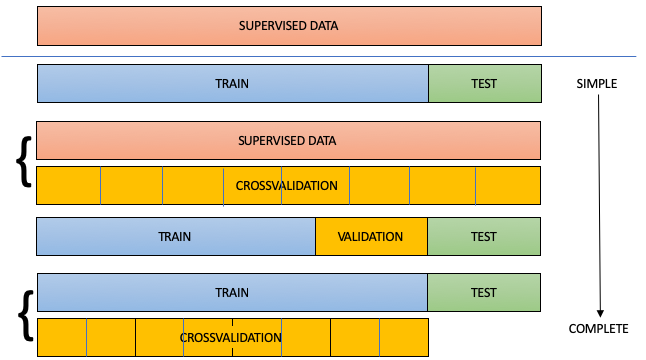
\includegraphics[scale=0.5]{../images/test_train_process.png}
 \caption{\textit{The image show the most common practices in machine learning application to maintain top generalization performances.}}  
 \label{scheme}
\end{figure}

Other causes for overfitting may come from the dataset: 

\begin{itemize}
 \item [-] individuals in the test set can have bad values in the predicting attributes
           and/or in the class label
 \item [-] Lack of representative instances some situations of the real world can be underrepresented, or not represented at all, in the training set. This situation is quite common.
\end{itemize}

As a rule, a good hypothesis has low generalization error i.e. it works well on examples different from those used in training.
\\
\\
In traditional machine learning methods, the "U-shaped" risk curve in figure \ref{bias-variance-tradeoff} is used to measure the bias-variance trade-offs and quantify how generalizable a model is \cite{weng2019overfit}.
As the model turns larger (more parameters added), the training error decreases to close to zero, but the test error (generalization error) starts to increase once the model complexity grows to pass the threshold between “underfitting” and “overfitting”

\begin{figure}[H]
 \centering
 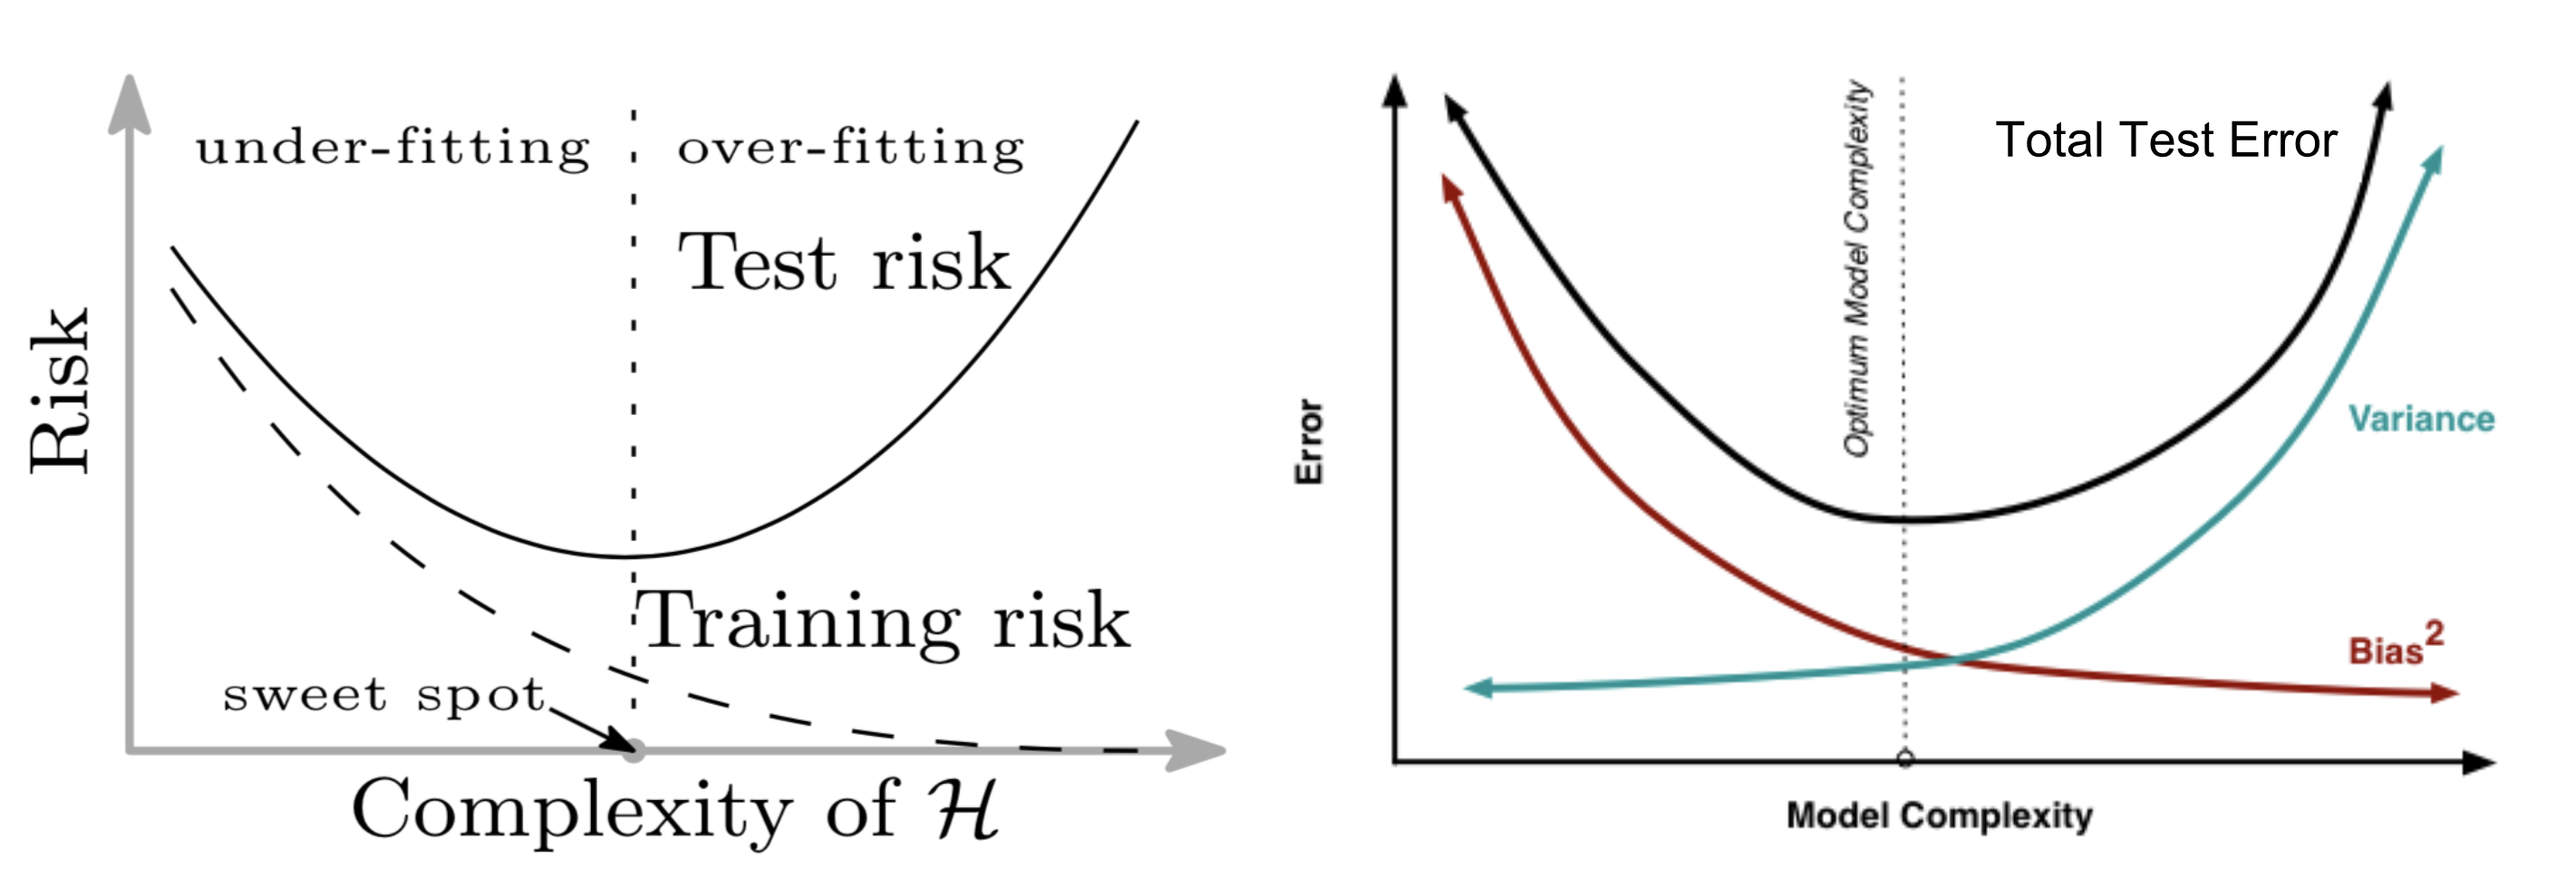
\includegraphics[scale=0.3]{../images/bias-variance-risk-curve.png}
 \caption{\textit{Classical view on Bias-Variance Trade-off in deep learning. The ideally trained model comes from a balance between under-fitting and over-fitting. Images from \cite{doubleU}}}  
 \label{bias-variance-tradeoff}
\end{figure}

\section*{Overfitting in Deep Learning}

In deep learning, overfitting is essentially threated the same as for other machine learning metods. 
It's easy to see how overfitting can appear in simple applications: in figure \ref{cifar-overfit-loss} is shown the charateristic trend of the loss in a overfitting model. 

\begin{figure}[H]
 \centering
 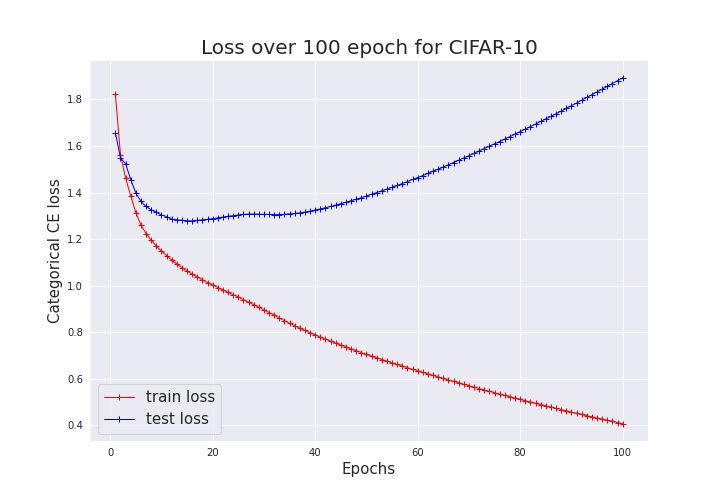
\includegraphics[scale=0.4]{../images/cifar10_100epochs_loss.png}
 \caption{\textit{The image shows a common overfitting behaviour in Deep Learning Applications. The cross entropy loss for the training set keeps a steady descent while the test set loss start increasing.}}  
 \label{cifar-overfit-loss}
\end{figure}

In this case, the Gradient Descent is performed on the categorical crossentropy loss, defined as : 

\begin{equation}
  CE = -\sum_{i=1}^{classes} t_i log(x_i)
\end{equation}

Where $t_i$ is the true label of the input, while $x_i$ is the predicted label of the input.
As shown in the graph below, it is clear how, if not monitored, overfitting can and does lead to contradictory results (very good on training set, very bad on test set). 


In figure \ref{cifar-overfit-error} is reported the behaviour of the classification error in the same experiment. The trend is clearly different from the previous one and the error stays more or less constant after the model reaches the mininum. 

\begin{figure}[H]
  \centering
  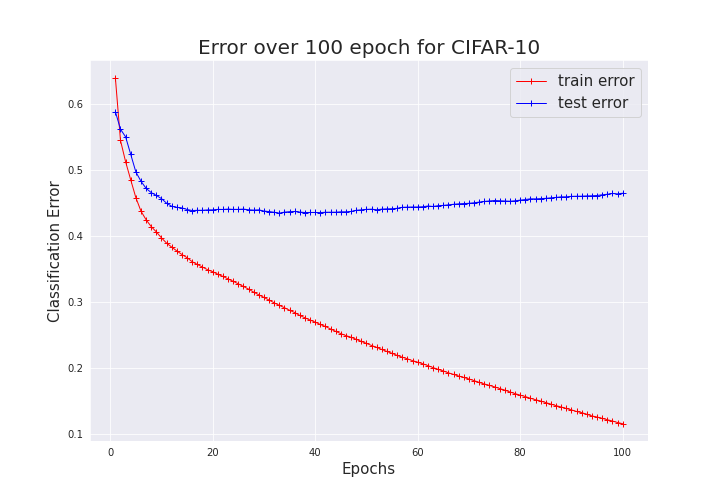
\includegraphics[scale=0.4]{../images/cifar10_100epochs_error.png}
  \caption{\textit{The image shows a common overfitting behaviour in Deep Learning Applications. The classification error in the test set remains almost constant while the classification error in the training set tends to zero after the "sweet spot"}}
  \label{cifar-overfit-error}
\end{figure}

The difference in the two graphs is one of the main reasons why accuracy is not a good target function while training deep learning model and, in general, to report machine learning results. Indeed, it only compares a predicted score $t$ to some cutoff $c$, which is not a proper scoring rule and conceals important information about model fitness.
Improper scoring rules such as proportions accuracy, sensitivity, and specificity are not only arbitrary (in choice of threshold) but are improper, i.e., they have the property that maximizing them leads to bad models, inaccurate predictions, and selecting the wrong features. 

Cross-entropy loss is more viable than accuracy because it is sensitive to "how wrong" the results are: if the label is $1$, but $t=0.9$, the cross-entropy is lower than when the label is $1$ but $t=0.1$.
The phenomenon when comparing these two graphs, accuracy is flat but loss is increasing, happens because $t>c$.

\section*{Recent Development}

In recent year, the view on overfitting in Deep Learning applications is drastically changing and this is due to new development in the theory of learning.
Practitioners routinely use modern machine learning methods, such as large neural networks and other non-linear predictors that have very low or zero training risk. In spite of the high function class capacity and near-perfect fit to training data, these predictors often give very accurate predictions on new data. Indeed, this behavior has guided a best practice in deep learning for choosing neural network architectures, specifically that the network should be large enough to permit effortless zero loss training (called interpolation) of the training data. Moreover, in direct challenge to the bias-variance trade-off philosophy, recent empirical evidence indicates that neural networks and kernel machines trained to interpolate the training data obtain near-optimal test results even when the training data are corrupted with high levels of noise. \cite{doubleU}.

In figure \ref{bias-variance-tradeoff-new} is shown the new Risk-Model Complexity curve proposed from the authors of the paper.

\begin{figure}[H]
 \centering
 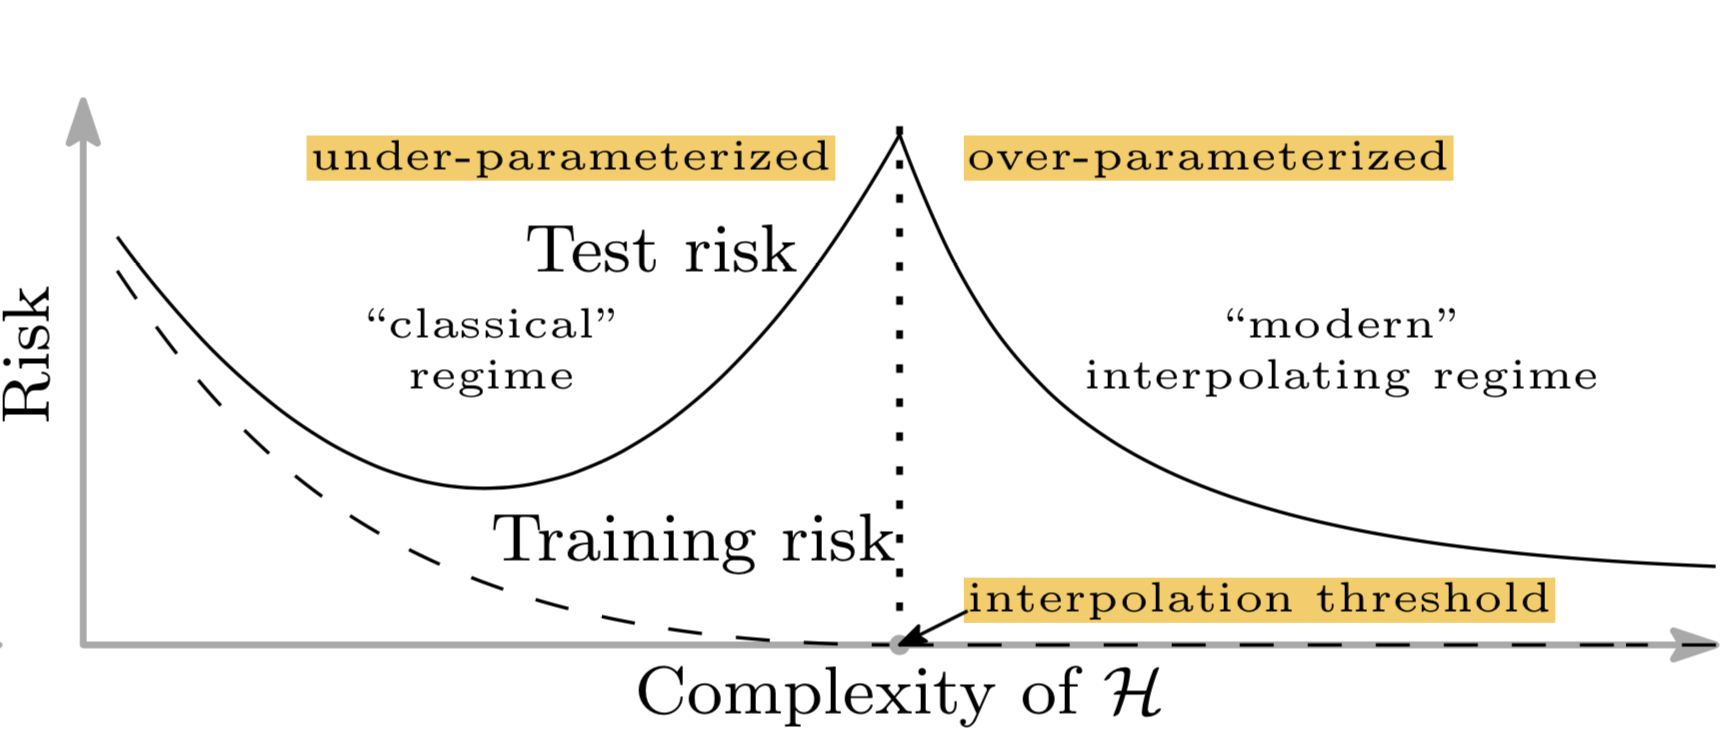
\includegraphics[scale=0.5]{../images/new-curve.png}
 \caption{\textit{New bias-variance curve proposed in \cite{doubleU}.}}  
 \label{bias-variance-tradeoff-new}
\end{figure}

The double descent risk curve, which incorporates te U-shaped risk curve ("classical regime") with the observed behaviour from using high capacity function classes ("modern regime"), seprated by a interpolation threshold. The predictors to the right have zero training risk.

In figure \ref{mnist-b-v} is shown the loss and the miss-classification error during the training of a one hidden-layer fully-connected neural network as a function of the

\begin{figure}[H]
 \centering
 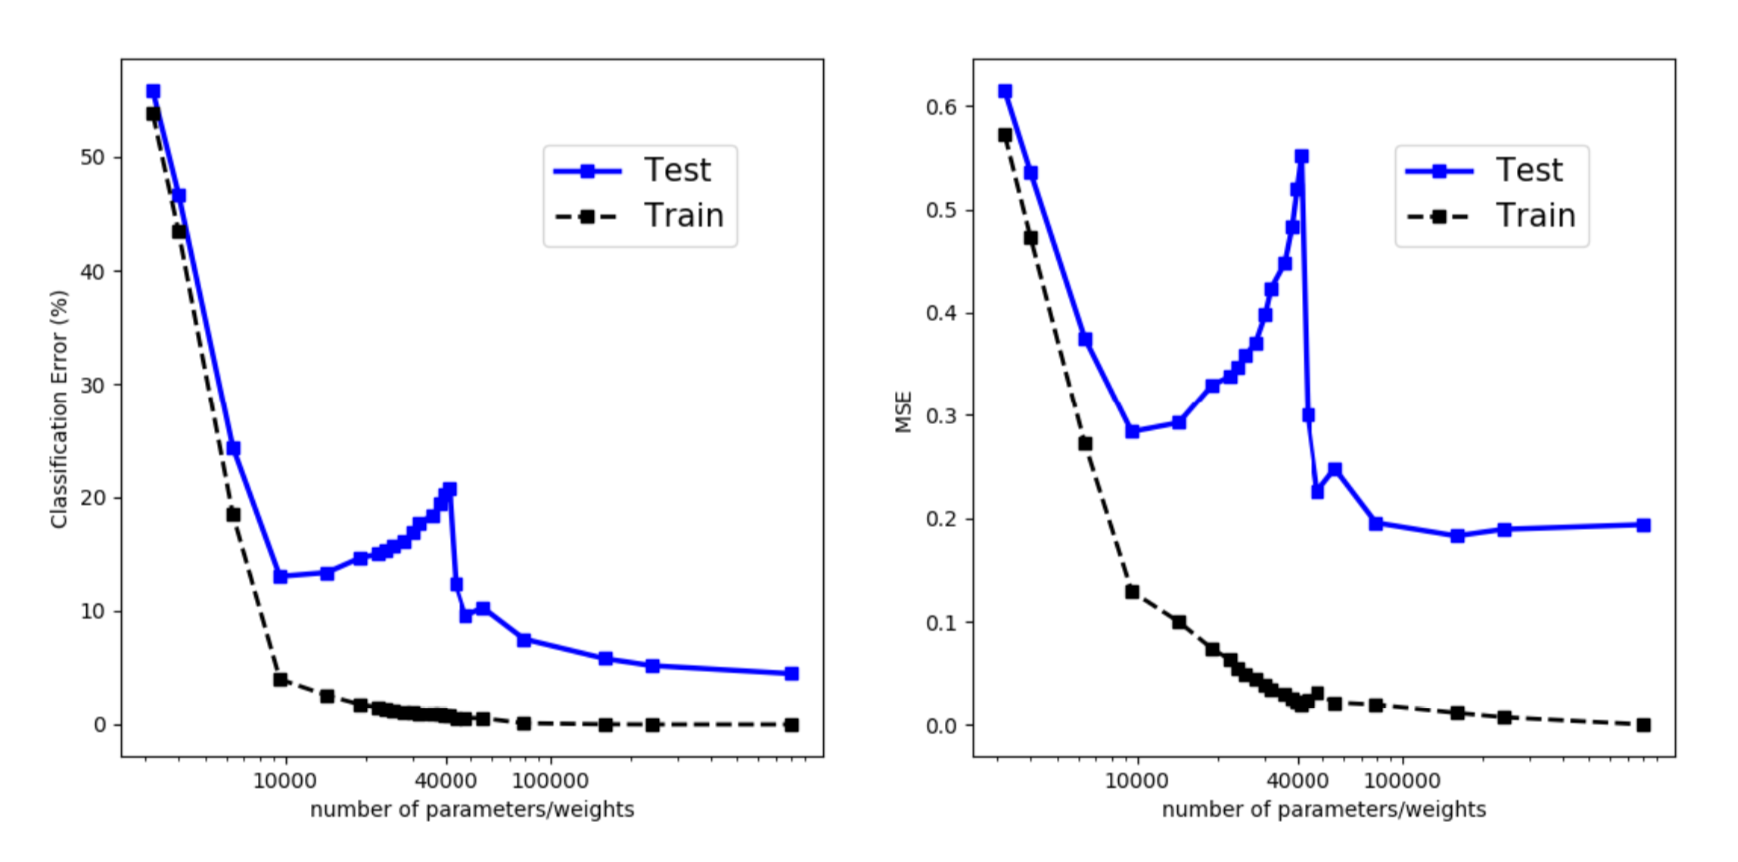
\includegraphics[scale=0.4]{../images/new-risk-curve-graph.png}
 \caption{\textit{Training and evaluation errors of a one hidden layer fc network of different numbers of hidden units, trained on 4000 data points sampled from MNIST. From \cite{doubleU}}}  
 \label{mnist-b-v}
\end{figure}

The paper claimed it is likely due to two reasons : 

\begin{itemize}
 \item [-] The number of parameters is not a good measure of inductive bias, defined as the set of assumptions of a learning algorithm used to predict for unknown samples.
 
 \item [-] Equipped with a larger model, we might be able to discover larger function classes and further find interpolating functions that have smaller norm and are thus “simpler”.
\end{itemize}

Regularization is a common way to control overfitting and improve model generalization performance. 
Interestingly some research \cite{rethink} has shown that explicit regularization (such as data augmentation, weight decay and dropout) is neither necessary or sufficient for reducing generalization error.

\begin{figure}[H]
 \centering
 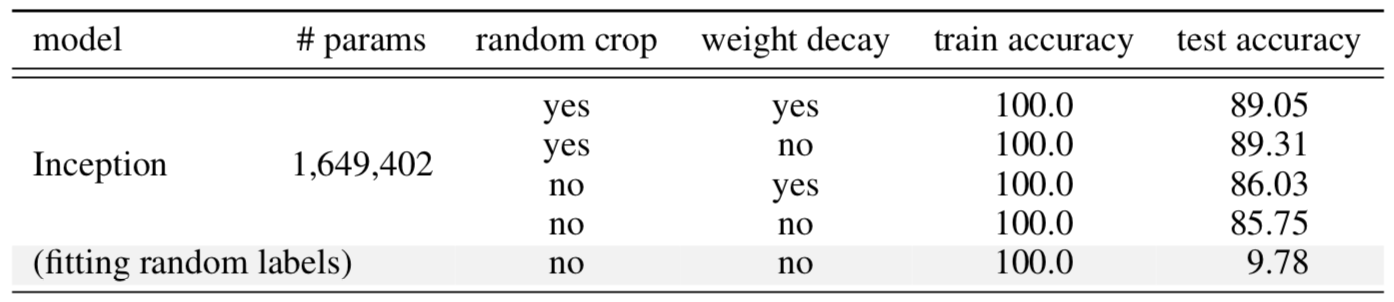
\includegraphics[scale=0.55]{../images/table_regul.png}
 \caption{\textit{The training and test accuracy (percentage) of Inception models on the CIFAR10 dataset (in the original paper more models are considered).
  Performance with and without data augmentation and weight decay are compared. The results of fitting random labels are also included. From \cite{rethink}.}}  
 \label{table}
\end{figure}

Two-layer neural networks are universal approximators, so given a sufficiently complex structure, they are able to learn any function. 
It has been proven that they are able to learn unstructured random noise as well, as shown in \cite{rethink} and \cite{Mit-overfit}. 
If labels of image classification dataset are randomly shuffled, the high expressivity power of deep neural networks can still empower them to achieve near-zero training loss. 
These results do not change with regularization terms added. 
Figure \ref{random-labels} shows some example of this behaviour.

\begin{figure}[H]
 \centering
 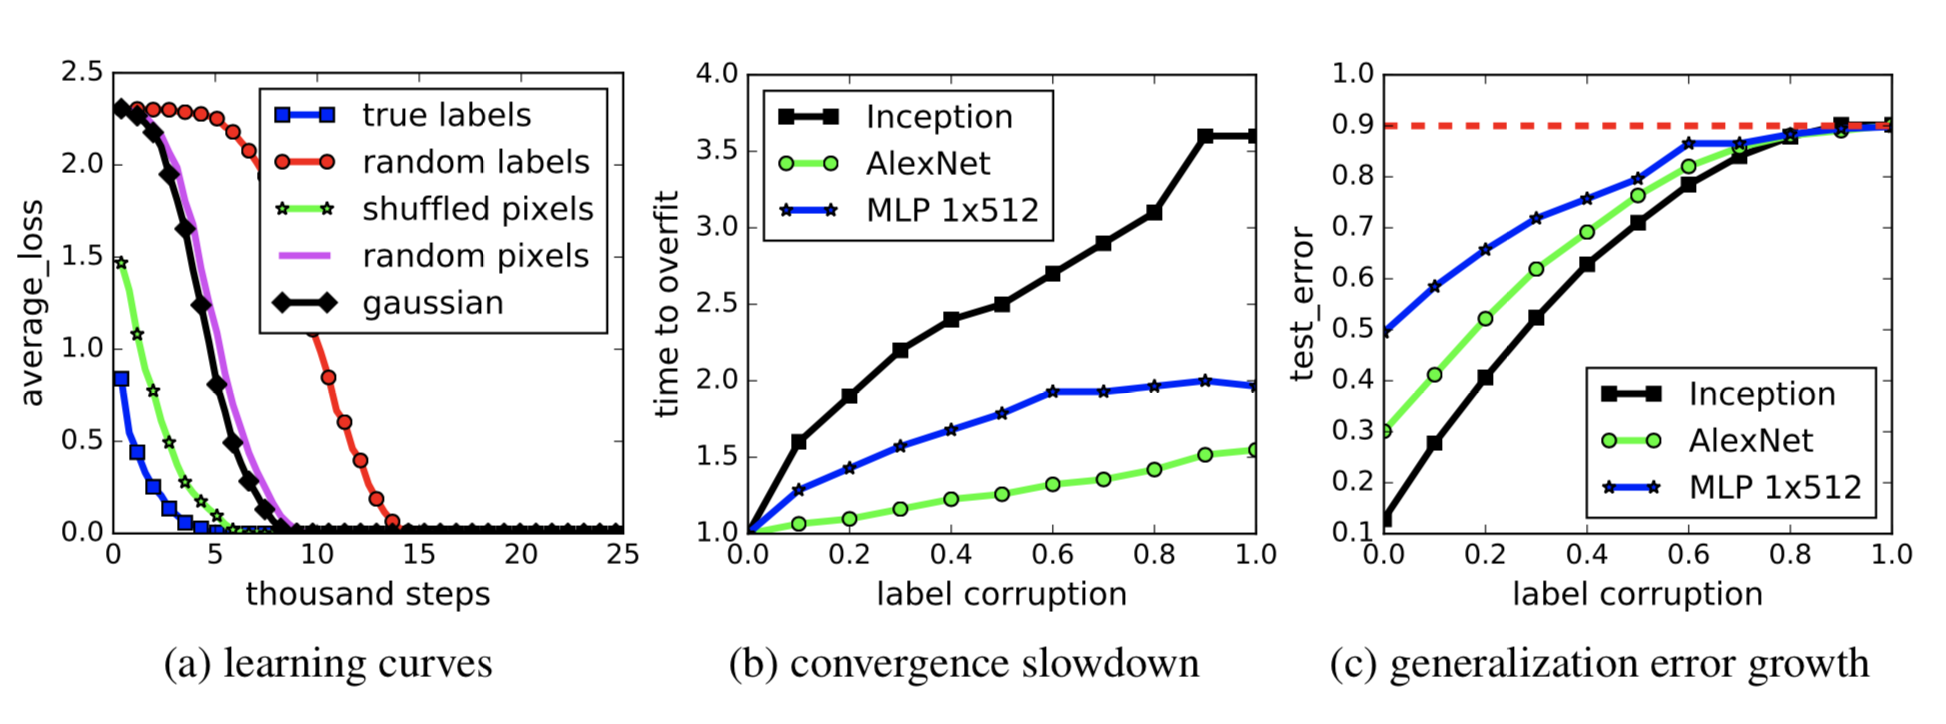
\includegraphics[scale=0.46]{../images/fit-random-labels-zhang.png}
 \caption{\textit{Fit models on CIFAR10 with random labels or random pixels: (a) learning curves; (b-c) label corruption ratio is the percentage of randomly shuffled labels. Image from \cite{rethink}}}  
 \label{random-labels}
\end{figure}

An interesting interpretation of those behaviour is given by the lottery ticket hypothesis \cite{lottery}. The article states that only a subset of network parameters have impact on the model performance and thus the network is not overfitted. The lottery ticket hypothesis suggest that a randomly initialized, dense, feed-forward network contains a pool of subnetworks and among them only a subset are “winning tickets” which can achieve the optimal performance when trained in isolation. Namely : 
\\
\\
``{\bf The Lottery Ticket Hypothesis.} {\it A randomly-initialized, dense neural network contains a subnetwork that is initialized such that — when trained in isolation — it can match the test accuracy of the original network after training for at most the same number of iterations.}'' \cite{lottery}
\\
\\
The paper identify a method to find "winning tickets" : 

\begin{enumerate}
 \item random initialization of a neural network with parameters $\theta_0$
 \item Train the net for $j$ iterations, reaching state $\theta_j$
 \item Prune a percentage of parameters $\theta_j$.
 \item Reset remaning parameters to values in $\theta_0$, creating the winning ticket
\end{enumerate}

The authors successfully found "winning tickets" for fully-connected and convolutional structure for MNIST and CIFAR-10 across different optimization strategy (SGD, Momentum and Adam). This hypothesis opens up new ways about interpreting deep neural networks results.



\newpage
\nocite{*}
\bibliographystyle{abbrv}
\bibliography{biblio}

\end{document}
